\documentclass[10pt,a4paper]{amsart}
\usepackage[margin=19mm]{geometry}
\usepackage{amsmath,amssymb,mathtools}
\usepackage[scr=rsfs,cal=euler]{mathalfa}
\usepackage{xfrac}
\usepackage[unicode,hidelinks,bookmarks=false]{hyperref}
\newcommand{\ie}{i.e.\ }
\newcommand{\cf}{cf.\ }
\newcommand{\resp}{respectively\ }
\newcommand{\Subsection}{\subsection}
\providecommand{\nobreakdash}{\nobreak\hbox{-}}
\setlength{\emergencystretch}{2em}
\multlinegap0pt
\usepackage{tikz}
\usepackage{amssymb}
\usepackage{enumerate}
\usepackage{float}
\usepackage{mathtools}
\usepackage{xcolor}
\newtheorem{theorem}{Theorem}
\newtheorem{lemma}{Lemma}
\newcommand{\tn}[1]{\textnormal{#1}}
\title{The $k$-Plancherel Measure and a Finite Markov Chain}
\author{Svante Linusson, Alperen \"Ozdemir}
\date{Source: arXiv:2512.24346v1 (CC BY 4.0)}
\begin{document}
\maketitle

\noindent\emph{Source and licence.} The $k$-Plancherel Measure and a Finite Markov Chain. Version arXiv:2512.24346v1 (CC BY 4.0), distributed by arXiv under the Creative Commons Attribution 4.0 International licence, http://creativecommons.org/licenses/by/4.0/, as recorded in the arXiv licence metadata for this exact version and shown on the abstract page https://arxiv.org/abs/2512.24346v1. Full licence notice: \texttt{licenses/arxiv-2512.24346-CC-BY-4.0.txt}.\par\smallskip

\noindent\textit{Editorial scope.} Counted unit: the article's lemma triangle-lemma (source0.tex lines 830--832). The article's complete original proof of it is delivered with it (source0.tex lines 834--946, one \texttt{proof} environment of 113 lines). No mathematics is written, repaired or re-derived: the statement and the proof are the article's own lines, in the article's own notation, and no retained line is substituted or re-flowed.  Retained uncounted as the source-local context the proof needs: lines 750--753.  Nothing was omitted from any retained span, so the package carries no omission record.  No retained line contains a citation, so the wrapper carries no bibliography and no bibliography entry.  The retained lines contain the article's own diagram code, which the wrapper typesets with the standard tikz packages; no image file is delivered and the package declares no asset dependency.  Editorial formatting only, in addition: an AMS \texttt{amsart} preamble that restates the article's own declarations and macros used by the retained lines, namely the environments \texttt{theorem}, \texttt{lemma} on separate counters, together with the standard packages those lines need.  The retained environments print in this document as Theorem 1, Lemma 1 in order of appearance, whereas the article prints the same items with the numbering of its own full document.  The complete native source of the article as distributed in the arXiv e-print for this exact version is bundled unchanged as \texttt{sources/191882/source0.tex}.
\begin{theorem}\label{thm:inversions} For every $t\ge 2$,
    \[\mathbf{R}^\triangle_t=\sum_{\pi\in S_{t}} (-1)^{|Inv(\pi)|}\prod_{(i,j)\in Inv(\pi)} R_{i,j}
    \]
\end{theorem}

\begin{lemma} \label{triangle-lemma}
Let $\mu \in \mathbb{Z}_+^{t+1}.$ If $\hat{\mu}=(\hat{\mu}_1,\ldots,\hat{\mu}_{t+1})=(0,\ldots,0,m)$ such that $1 \leq m \leq t,$ we have $\mathbf{R}^\triangle_{t}(\mu)=0.$ 
\end{lemma}

\begin{proof} The proof is by induction over $t$. For all $t,$ we distinguish the two cases: (1) $1 \leq m \leq t-1$ and (2) $m=t$.

For $t=1,$ the only possibility is $\hat{\mu}=(0,1),$ and $\mathbf{R}^\triangle_1=\{R_{12}\}.$ Therefore we match $(1,0)$ with $(0,1)$ where we apply $R_{12}$ in the former and do not apply any non-trivial operator in the latter. Since the parities differ by one, they cancel out each other. 

Suppose $t\geq 2,$  and consider the three regions for the operators:\\
The top-left triangle is 
\[T:= \left\{ (i,j) \in \mathbb{Z}^2_{+} \, : \,  t-m+1 \leq i \leq t , i+1 \leq j \leq t+1 \right\}.\]
Then we have the bottom triangle
\[D:= \left\{ (i,j) \in \mathbb{Z}^2_{+} \, : \,  1 \leq i \leq t-m-1 , i+1 \leq j \leq t-m \right\}.\]
Finally, we have the strip 
\[S:= \left\{ (i,j) \in \mathbb{Z}^2_{+} \, : \,  1 \leq i \leq t-m , t-m+1 \leq j \leq t+1 \right\},\]
see Figure \ref{triangle}. Note that the regions above define the labels of the associated operators, not the actual regions in the figure, and that the sum of the combinations of operators in $T$ is just $\mathbf{R}_{m}^{\triangle}$ shifted by $t-m$. 

\begin{figure} 
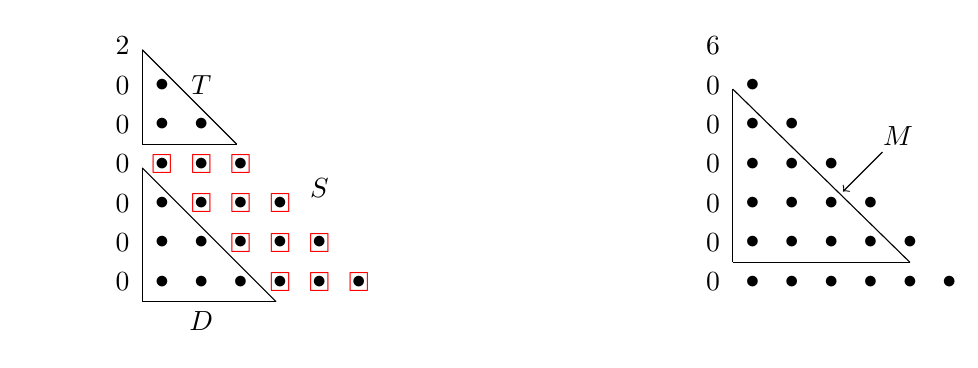
\begin{tikzpicture}
\hspace*{1cm}

  \foreach \y in {1,1.5,...,3} {
        \draw (0, \y -1) node{$0$} ++(1,1);
    \foreach \x in {0.5,1,...,\y} {
      \draw (\x, 3-\y) node{$\bullet$} ++(1,1);
          }
  }
  
  \foreach \x in {0,0.5,1} {
    \foreach \y in {0,0.5,1,1.5} {
      \draw (2+\x-\y, \y) node{$\color{red}\square$} ++(1,1);
          }
  }

       \draw (0.5, 2.5) node{$\bullet$};
       \draw (0, 2.5) node{$0$}; 
       \draw (0, 3) node{$2$} ;
              \draw (1, 2.5) node{$T$} ;
              \draw (1, -0.5) node{$D$} ;
              \draw (2.5, 1.2) node{$S$} ;


     
      \draw (0.25,1.75) -- (1.45,1.75);
\draw (0.25,1.75) -- (0.25,2.95);
\draw (0.25,2.95) -- (1.45,1.75);

\draw (0.25,-0.25) -- (0.25,1.45);
\draw (0.25,-0.25) -- (1.95,-0.25);
\draw (0.25,1.45) -- (1.95,-0.25);

 \foreach \y in {1,1.5,...,3} {
        \draw (7.5, \y -1) node{$0$} ++(1,1);
    \foreach \x in {0.5,1,...,\y} {
      \draw (7.5+\x, 3-\y) node{$\bullet$} ++(1,1);
          }
  }


 \draw (8, 2.5) node{$\bullet$};
       \draw (7.5, 2.5) node{$0$}; 
       \draw (7.5, 3) node{$6$} ;
     
 \draw (7.75,0.25) -- (10,0.25);
\draw (7.75,0.25) -- (7.75,2.45);
\draw (7.75,2.45) -- (10,0.25);

              \draw (9.85, 1.85) node{$M$} ;
\draw [->] (9.65,1.65) -- (9.15,1.15);


\end{tikzpicture}
\caption{An example for Lemma \ref{triangle-lemma}. $t=6$ and $m=2$ for the figure on the left while $t=m=6$ for the figure on the right.}
\label{triangle}
\end{figure}


 
Starting with the first case $m \leq t-1,$ the induction hypothesis implies that there exists a matching within $T$, that is to say, for all $X \subseteq T$ there exists a unique $X' \subseteq T$ such that
\begin{equation} \label{match}
 R_X(\mu) \leftrightarrow R_{X'}(\mu) = \pi(R_X(\mu))   
\end{equation}
for some $\pi \in \mathcal{S}_{m+1}.$ Note that we can choose $X'=X$ if $R_X$ is not applicable to $\mu.$ For example, if $\mu_j=1$, $X=\{(i_1,j),(i_2,j)\}$ and $(j,s)\notin X$ for any $s$,  then $R_X$ is not applicable to $\mu$ because there are no two boxes to displace at the $j$th part of $\mu.$ See 
Theorem \ref{thm:inversions} where $2^{\binom{n}{2}}-n!$ possible choices for subsets of operators that are not applicable.

 
Now we consider $Y \subseteq S.$ We first partition $Y$ with respect to the first coordinates of its elements; let $Y_l =Y \cap (\{l\}\times \mathbb{Z}_+).$ Then we define $\pi(Y_l)$, for the same $\pi\in S_{m+1}$ as above, by letting 
\[\pi(Y_l)=\{(l,j) \in S \, : \, (l,\pi^{-1}(j)) \in Y_l\}.\] 
 Observe that $R_{Y_l}$ and $R_{\pi(Y_l)}$ have the same parity, and we have the matching 
    \[R_{Y_1} \circ \cdots \circ R_{Y_{m-t}} \circ R_X(\mu)  +R_{\pi(Y_1)} \circ \cdots \circ R_{\pi(Y_{m-t})}  \circ \pi(R_X(\mu))=0.\]
 Then for any $Z \subseteq D,$ we can apply $R_Z$ to both sides of the matching above and it will still be a matching. Thus we are done with the first case.

Now we look at the case $m=t.$ We consider the operators in the middle of the triangle $T,$
\[M= \left\{(i,j) \in \mathbb{Z}^2_{+} \, : \,  2 \leq i \leq t-1 , i+1 \leq j \leq t \right\},\]
see the right image in Figure \ref{triangle}.
Then we look at the operators on the sides
\begin{align*}
K:&= \left\{ (i,t+1) \in \mathbb{Z}^2_{+}\, : \, 2 \leq i \leq t  \right\} \cup \left \{ (1,j) \in \mathbb{Z}^2_{+} \, : \, 2 \leq j \leq t-1\right\} \cup \{(1,t)\} \\
&= \left\{(2,t+1),(3,t+1),\ldots, (t,t+1),(1,2),(1,3),\ldots, (1,t-1), (1,t) \right \}.
\end{align*}

For any $X \subseteq M$ and $Y \subseteq K,$ we will find some $Y' \in K$ such that
\[R_Y \circ R_X (\hat{\mu}) + R_{Y'} \circ R_X (\hat{\mu}) = 0.\]

Note that $X$ will not alter the top part nor the bottom part. The bottom part of 
$R_Y \circ R_X (\hat{\mu})$ will be equal to the number of $R_{1j}\in Y$ and the size of the top part will be $t$ minus the number of $R_{it}\in Y$. Boxes can be moved from the top part to the bottom part by  pairs 
$R_{1,i}R_{i,t+1}, 2\le i\le t-1$ and by $R_{1,t+1}$. We construct $Y'$ by interchanging all pairs $R_{1,i}R_{i,t+1}$ and also $R_{1,t+1}$ to change the parity. This gives the same partition with top and bottom parts interchanged and reverse parity.
In symbols $Y'$ is constructed as follows. For $i=2,\ldots, t,$
\begin{align*}
\tn{ If } &\left\{(i,t+1), (1, i)\right\} \subseteq Y, \tn{ then }  \left\{(i,t+1), (1, i)\right\} \cap Y'=\emptyset,\\
\tn{ while if } &\left\{(i,t+1), (1, i)\right\} \cap Y = \emptyset, \tn{ then }  \left\{(i,t+1), (1, i)\right\} \subseteq Y',\\
\tn{ otherwise } &\left\{(i,t+1), (1, i)\right\} \cap Y = \left\{(i,t+1), (1, i)\right\} \cap Y'.
\end{align*}
Finally, we take 
\[(1,t) \in Y \tn{ if and only if }(1,t) \notin Y'.\]
This last step guaranties $R_Y$ and $R_{Y'}$ have different parities. This completes the inductive step and the proof.
\end{proof}

\end{document}
